\documentclass[tikz,border=5pt]{standalone}
\usepackage{amsmath,amssymb}
\usetikzlibrary{arrows.meta,positioning,calc}
\begin{document}
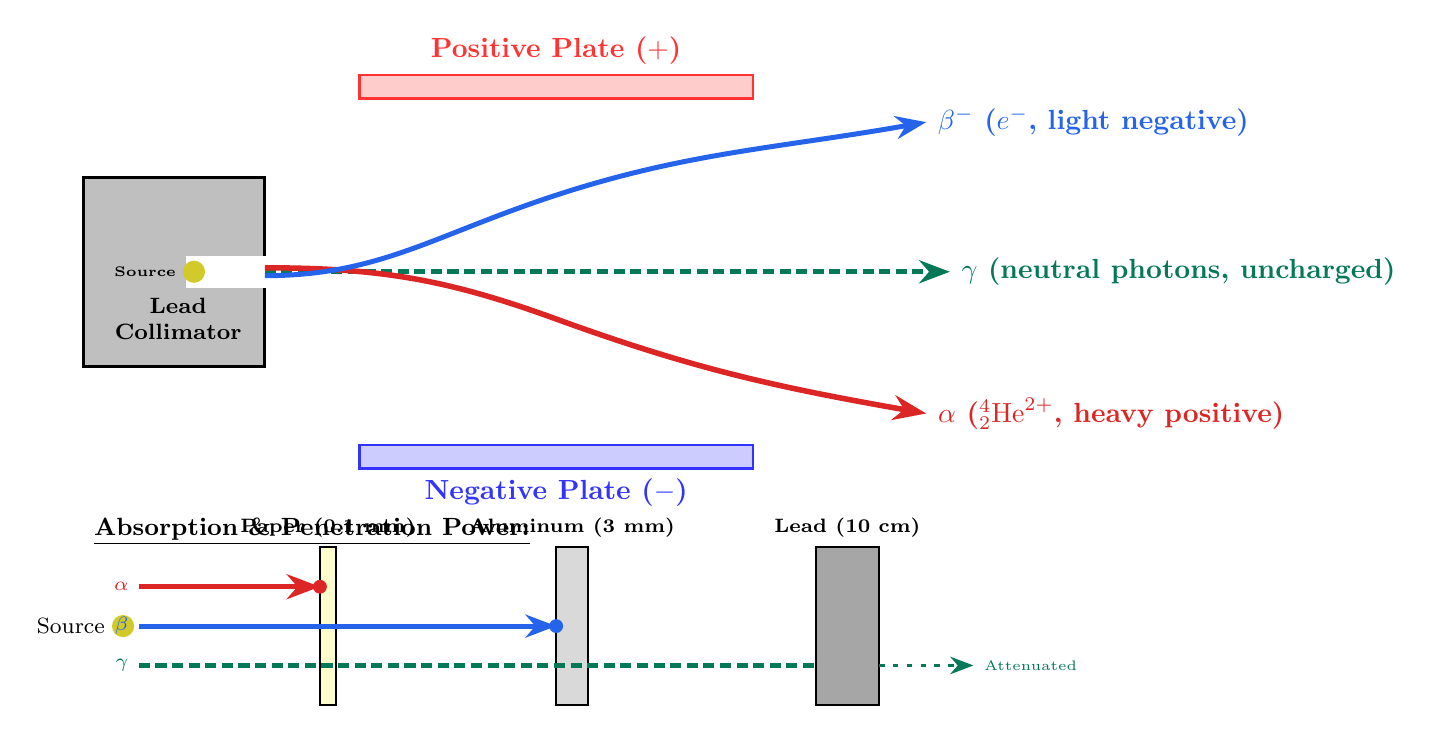
\begin{tikzpicture}[>=Stealth, font=\sffamily, thick]
  \definecolor{alphacolor}{HTML}{DC2626}
  \definecolor{betacolor}{HTML}{2563EB}
  \definecolor{gammacolor}{HTML}{047857}

  % Electric Field Plates
  \fill[red!20, draw=red!80, line width=1pt] (2, 2.2) rectangle (7, 2.5);
  \node[above, text=red!80, font=\bfseries] at (4.5, 2.5) {Positive Plate ($+$)};

  \fill[blue!20, draw=blue!80, line width=1pt] (2, -2.5) rectangle (7, -2.2);
  \node[below, text=blue!80, font=\bfseries] at (4.5, -2.5) {Negative Plate ($-$)};

  % Radioactive Lead block
  \fill[gray!50, draw=black, line width=1.2pt] (-1.5, -1.2) rectangle (0.8, 1.2);
  \fill[white] (-0.2, -0.2) rectangle (0.85, 0.2);
  \node[font=\footnotesize\bfseries, align=center] at (-0.3, -0.6) {Lead\\Collimator};
  \fill[yellow!80!black] (-0.1, 0) circle (4pt);
  \node[left, font=\tiny\bfseries] at (-0.2, 0) {Source};

  % Rays
  % Gamma (undeflected)
  \draw[->, line width=1.8pt, gammacolor, dash pattern=on 4pt off 2pt] (0.8, 0) -- (9.5, 0) node[right, font=\bfseries] {$\gamma$ (neutral photons, uncharged)};

  % Alpha (deflected toward negative plate, gentle curvature)
  \draw[->, line width=2pt, alphacolor] (0.8, 0.05) to[out=0, in=160] (4.5, -0.6) to[out=-20, in=170] (9.2, -1.8) node[right, font=\bfseries] {$\alpha$ ($^4_2\mathrm{He}^{2+}$, heavy positive)};

  % Beta (deflected toward positive plate, sharp curvature)
  \draw[->, line width=1.8pt, betacolor] (0.8, -0.05) to[out=0, in=200] (4.0, 0.8) to[out=20, in=190] (9.2, 1.9) node[right, font=\bfseries] {$\beta^-$ ($e^-$, light negative)};

  % Penetration barriers below
  \begin{scope}[shift={(0, -4.5)}]
    \node[anchor=west, font=\bfseries\small] at (-1.5, 1.2) {\underline{Absorption \& Penetration Power:}};
    
    % Source
    \fill[yellow!80!black] (-1.0, 0) circle (4pt);
    \node[left, font=\footnotesize] at (-1.1, 0) {Source};

    % Barriers
    % Paper
    \fill[yellow!20, draw=black] (1.5, -1.0) rectangle (1.7, 1.0);
    \node[above, font=\scriptsize\bfseries] at (1.6, 1.0) {Paper (0.1 mm)};

    % Aluminum
    \fill[gray!30, draw=black] (4.5, -1.0) rectangle (4.9, 1.0);
    \node[above, font=\scriptsize\bfseries] at (4.7, 1.0) {Aluminum (3 mm)};

    % Lead
    \fill[gray!70, draw=black] (7.8, -1.0) rectangle (8.6, 1.0);
    \node[above, font=\scriptsize\bfseries] at (8.2, 1.0) {Lead (10 cm)};

    % Alpha stopped by paper
    \draw[->, line width=2pt, alphacolor] (-0.8, 0.5) -- (1.5, 0.5);
    \node[left, font=\scriptsize\bfseries, alphacolor] at (-0.8, 0.5) {$\alpha$};
    \fill[alphacolor] (1.5, 0.5) circle (2.5pt);

    % Beta stopped by aluminum
    \draw[line width=1.8pt, betacolor] (-0.8, 0.0) -- (1.7, 0.0);
    \draw[->, line width=1.8pt, betacolor] (1.7, 0.0) -- (4.5, 0.0);
    \node[left, font=\scriptsize\bfseries, betacolor] at (-0.8, 0.0) {$\beta$};
    \fill[betacolor] (4.5, 0.0) circle (2.5pt);

    % Gamma penetrates lead partially
    \draw[line width=1.8pt, gammacolor, dash pattern=on 4pt off 2pt] (-0.8, -0.5) -- (7.8, -0.5);
    \draw[->, line width=1.2pt, gammacolor, dash pattern=on 2pt off 3pt] (8.6, -0.5) -- (9.8, -0.5) node[right, font=\tiny] {Attenuated};
    \node[left, font=\scriptsize\bfseries, gammacolor] at (-0.8, -0.5) {$\gamma$};
  \end{scope}
\end{tikzpicture}
\end{document}
